% GENERATED — do not edit by hand.
% script : scripts/gen_figures.py
% source : /home/rohit/sprs-fix/data/results/live_hw_results_p1_maxpe.csv
% metric : max over PEs (corrected)
% date   : 2026-09-08
% Colours: Okabe-Ito colourblind-safe. Marker shape duplicates hue
% so the figure survives greyscale printing.

\definecolor{ctorus}{HTML}{0072B2}
\definecolor{cfattree}{HTML}{D55E00}
\definecolor{chypercube}{HTML}{009E73}
\definecolor{cring}{HTML}{CC79A7}
\definecolor{cmesh}{HTML}{E69F00}
\definecolor{clinear}{HTML}{000000}

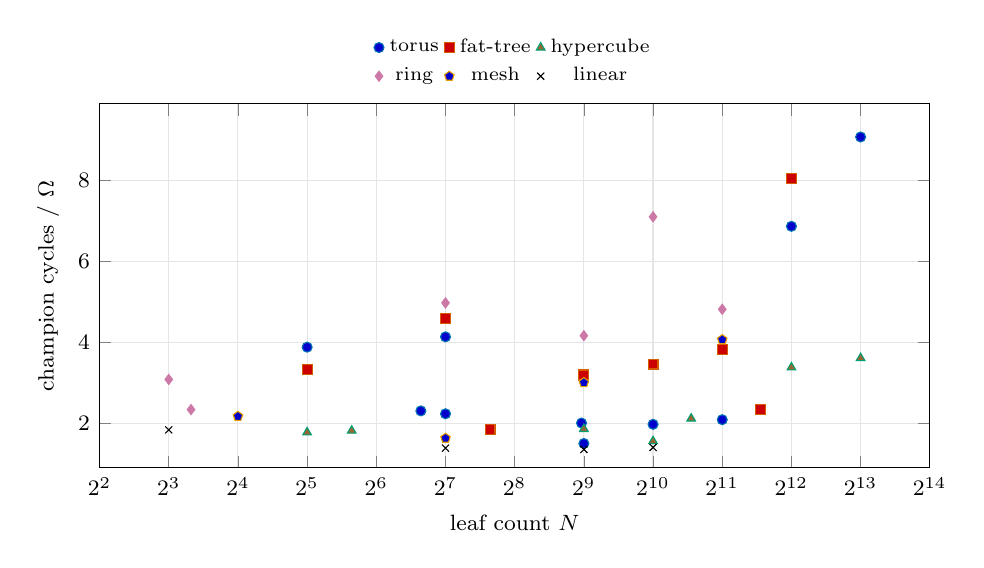
\begin{tikzpicture}
\begin{axis}[
  width=\columnwidth, height=6.2cm,
  xmode=log, log basis x=2,
  xlabel={leaf count $N$}, ylabel={champion cycles $/\ \Omega$},
  ymin=0.9,
  grid=major, major grid style={gray!20},
  legend style={font=\scriptsize, at={(0.5,1.02)}, anchor=south,
                legend columns=3, draw=none, fill=none},
  tick label style={font=\footnotesize},
  label style={font=\footnotesize},
  mark options={scale=0.9}]
\addplot+[only marks, mark=*, color=ctorus] coordinates {(32,3.875) (100,2.300) (128,2.229) (128,4.130) (500,2.000) (512,1.495) (1024,1.969) (2048,2.083) (4096,6.861) (8192,9.068)};
\addlegendentry{torus}
\addplot+[only marks, mark=square*, color=cfattree] coordinates {(32,3.333) (128,4.583) (200,1.833) (512,3.188) (1024,3.458) (2048,3.812) (3000,2.340) (4096,8.043)};
\addlegendentry{fat-tree}
\addplot+[only marks, mark=triangle*, color=chypercube] coordinates {(32,1.771) (50,1.812) (512,1.854) (1024,1.552) (1500,2.111) (4096,3.375) (8192,3.604)};
\addlegendentry{hypercube}
\addplot+[only marks, mark=diamond*, color=cring] coordinates {(8,3.077) (10,2.333) (128,4.969) (512,4.159) (1024,7.095) (2048,4.810)};
\addlegendentry{ring}
\addplot+[only marks, mark=pentagon*, color=cmesh] coordinates {(16,2.167) (128,1.625) (512,3.000) (2048,4.062)};
\addlegendentry{mesh}
\addplot+[only marks, mark=x, color=clinear] coordinates {(8,1.833) (128,1.380) (512,1.349) (1024,1.398)};
\addlegendentry{linear}
\end{axis}
\end{tikzpicture}
